\chapter{Further implementation key events}
\label{appendix4-further-implementation-key-events}
\graphicspath{{Appendix4/Figs/}{Appendix4/Figs/}}

This appendix lists other key events that took place during the 10 sprints of the project to create the next version of IDUN's NIP.

\section*{Python to WebAssembly}
\label{chapter4-python-to-webassembly}

Another key event during the 10 sprints took place about two sprints before evaluating the web-native approach. The idea was that, as mentioned in \autoref{chapter3-software-and-tools}, when it comes to how important and necessary the Python ecosystem is for IDUN and external people as presented in the personas, it might be possible to create Python code for specific neural signal data processing, compile it to WebAssembly (a low-byte compilation target for high-level languages that run mainly in the browser)  and then use it in web applications such as the GUI application of IDUN's NIP. Sprint 5 evaluated compiling Python into WebAssembly, which seemed promising at first but turned out to be too far removed from current capabilities. There is an interesting open-source project called RustPython—a Python interpreter written in Rust that allows the interpreted code to be compiled in WebAssembly. However, the project’s maturity is currently unsuitable for production \citep{noauthor_rustpython_2022}.

Another option would be to use Pyodide, which is the CPython interpreter ported to WebAssembly  \citep{noauthor_pyodide_2022}. Apart from the fact that the creation of a web application would be drastically more significant if a complete Python interpreter were sent to the browser, this interpreter also does not currently have the functionality to add additional Python packages apart from the standard library. This makes it easy to build vanilla Python on top of WebAssembly codebases, but not with custom packages installed, such as machine-learning packages needed for EEG classifiers. The only options left were to develop one’s own Python-to-WebAssembly compiler, contribute to the two open source projects, or give up the task of embedding Python code in a web application such as IDUN’s GUI application to interact with NIP’s API. The latter was chosen because it was still too early, immature, and time-consuming, as the results of Sprint 5 showed.

\section*{Kubernetes and Fargate}
\label{chapter4-kubernetes-and-aws-fargate}

One of the first technical decisions the author made involved which technology to use for creating backends for an n-tier\footnote{The term n-tier refers to an architecture design pattern where the logic of presentation, application processing, and data management are decoupled from each other, as in the case of multiple microservices.} system such as IDUN’s NIP. The use of a microservice approach was already established by the fact that a polyglot backend was needed, such as Python for data-heavy tasks and TypeScript for real-time and API-specific tasks due to the maturity in the previously mentioned examples of each language. If one decides to take a microservice approach, it can still be debated whether to proceed with serverless functions instead of hosting container images. Given the requirement to use AWS mentioned in \autoref{chapter3-software-and-tools}, the only way to host serverless functions was to use AWS Lambda. AWS Lambda was already used in the previous PoC version of the software system at IDUN and did not work as well as in cases where, for example, batch processing of previously collected data would exceed the maximum computation time or CPU limit of AWS Lambda. This limitation, coupled with the challenge of handling dozens if not hundreds of serverless functions and managing the entire collection of multiple functions and their versions and endpoints, led to the decision not to use Lambda for the most essential and critical parts of the backend in the author’s experience so far. Building microservices without serverless functions on AWS provides multiple solutions: the most prominent ones are utilising Kubernetes via AWS Elastic Kubernetes Service (EKS) or AWS Fargate, which is a serverless version of Kubernetes \citep{amazon_web_services_inc_serverless_nodate} that makes some parts of Kubernetes easier to handle, as shown in \autoref{fig:aws-fargate}.

\begin{figure}[!ht]
  \centering
  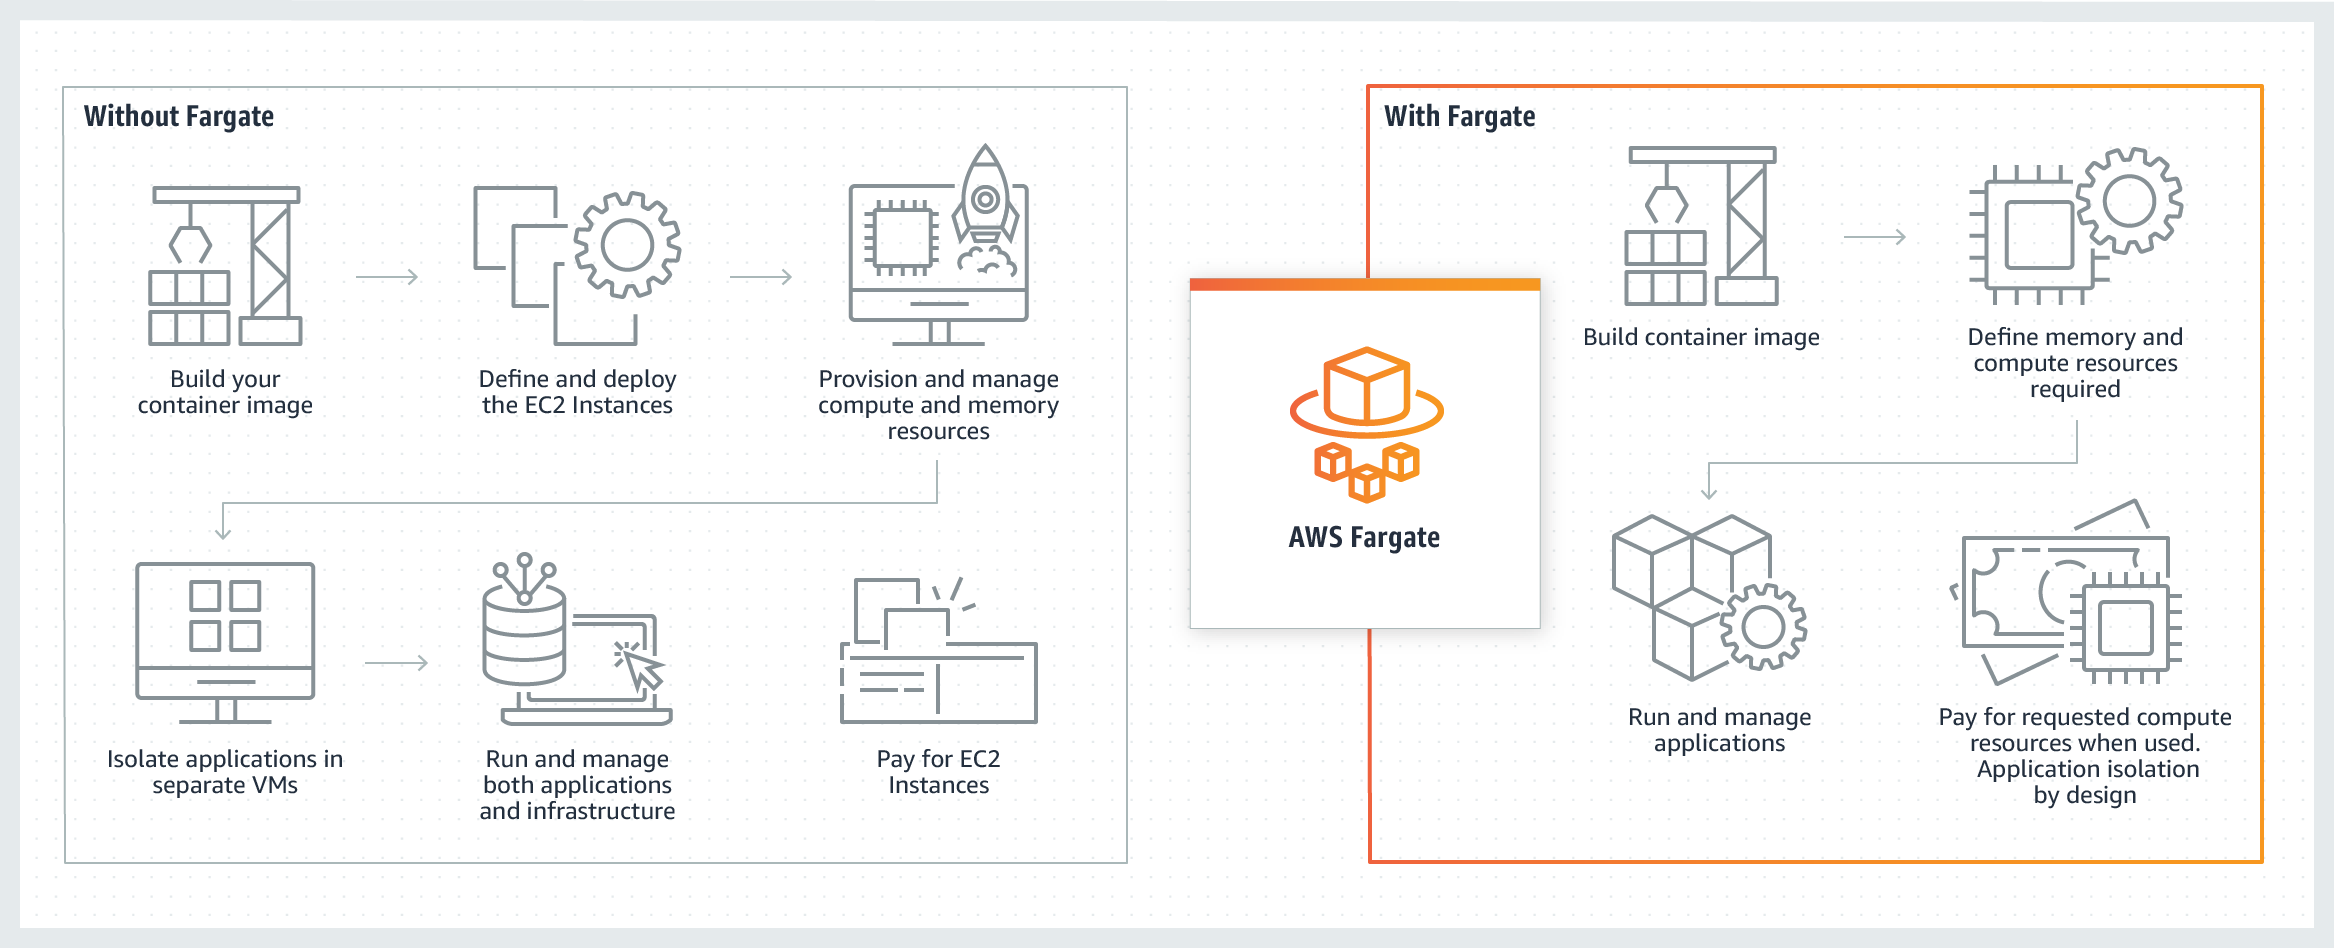
\includegraphics[width=\linewidth]{aws-fargate.png}
  \caption[Comparison of Fargate versus other container management tools]{Comparison of Fargate versus other container management tools \citep{amazon_web_services_inc_serverless_nodate}.}
  \label{fig:aws-fargate}
\end{figure}

The author consulted cloud experts in the first sprints from the company Nuvibit to guide the decision. The author himself is not experienced in Kubernetes and would need to learn many ways to implement a Kubernetes cluster, which was one of the items to avoid mentioned in \autoref{chapter3-software-and-tools}. Nuvibit recommended going with AWS Fargate since it is similar to Kubernetes but abstracts most things away to concentrate on adding business logic rather than handling the overheads that come with introducing a Kubernetes cluster. Fargate is also essentially serverless, making it cheaper for a product with hard-to-estimate usage such as IDUN’s NIP in the beginning; but it still gives enough flexibility in specifying the underlying hardware for computationally heavier tasks that would exceed AWS Lambda. As soon as IDUN moves toward large-scale deep learning models that utilise specific GPU units, Fargate will come to its limits since specifying GPU tasks is impossible \citep{amazon_web_services_inc_aws_2019}. One way or another, this decision will have to be reconsidered in the future to avoid a long-term commitment to one provider such as AWS and to the increasing investments of Kubernetes from several cloud providers.

\section*{Kafka and Kinesis}
\label{chapter4-kafka-aws-kinesis}

Another early technical decision, made with the help of expert interviews, concerned which streaming technology to use. As with many things in software, there are hundreds, if not thousands, of ways to solve a problem, such as streaming text-based data such as the EEG data from IDUN’s device over the internet to the cloud. Initially developed by LinkedIn, Apache Kafka is a prominent technology for such a use case. It is battle-tested, used in production by large technology companies \citep{apache_apache_nodate} and well maintained by an active community \citep{noauthor_apache_2022}. However, similar to Kubernetes, it comes with much overhead; moreover, the author himself has no experience with Kafka, so he would have to learn everything from scratch. Another option is to use AWS Kinesis, a service that AWS provides to process data streams over the cloud, as Kafka does, but without the overhead of managing the Kafka instances themselves. AWS Kinesis allows streams to be replayed, restored, and sent to an AWS Fargate cluster (e.g. real-time processing of the data) or data to be stored securely in storage systems such as AWS Simple Storage Service (S3), as shown in \autoref{fig:aws-kinesis}. One important aspect is that the data source can also come from a WebSocket stream, which will be addressed in the following section. However, the decision for Kinesis was relatively easy as the reasoning was similar to that between Kubernetes and AWS Fargate. The decision was also supported by the experience and opinion of the cloud experts at Nuvibit.

\begin{figure}[!ht]
  \centering
  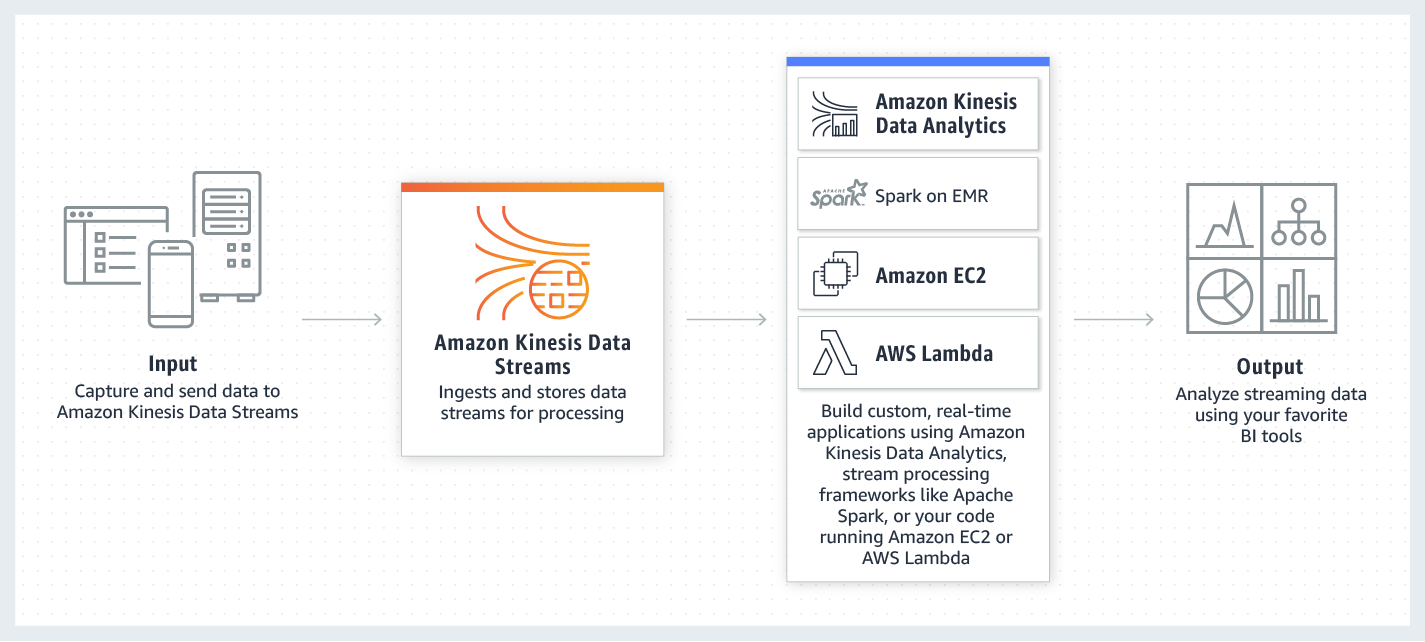
\includegraphics[width=\linewidth]{aws-kinesis.png}
  \caption[Example use-case architecture of AWS Kinesis]{Example use-case architecture of AWS Kinesis \citep{amazon_web_services_inc_amazon_nodate}.}
  \label{fig:aws-kinesis}
\end{figure}

\section*{MQTT and WebSocket}
\label{chapter4-mqtt-and-websocket}

As previously stated, a decision had to be made regarding the technology to transfer data from a physical device, such as IDUN’s EEG sensor hardware, to the cloud. Previous engineers at IDUN used MQTT to stream data from the hardware directly to the web app, as mentioned in the list of bugs and flaws in \autoref{chapter3-derivation-of-the-case-study}. MQTT is not well suited to sending high-frequency data in real-time, such as EEG, and it is geared toward lower-power IoT devices rather than, say, a computer or smartphone to which the IDUN device would be connected. As a result, the decision to use something else had to be considered. Another option is to use WebSocket, which is designed for high-frequency updates that can be up- dated in real-time in both directions. IDUN would want to use a high-frequency protocol because HTTP can only handle about ten requests per second, whereas WebSocket can handle nearly 4000 requests in the same amount of time. The main reason for this significant difference is that the browser limits the number of concurrent HTTP connections, whereas a WebSocket connection has no limit on the number of messages it can send or receive \citep{luecke_http_2018}. Sending EEG data at a frequency rate of 250 samples per second from the IDUN hardware and receiving multiple classification responses from the cloud based on the chosen classification necessitates more than ten requests per second.

WebSocket also integrates easily with the earlier technology decision for AWS Kinesis, as Kinesis can subscribe to an API gateway service from AWS that can be used to build Representational State Transfer (REST) APIs. (This is discussed in greater depth in \autoref{chapter5-example-architecture-of-an-nci}). An internal group discussion with firmware engineers for IDUN’s hardware was organised to validate this decision, as it was too BCI-specific to ask Nuvibit’s cloud engineers. The alignment with the firmware roadmap and its interface, which would be necessary for the BLE library that would consume it was key to the success of building an example N/CI at IDUN.

\section*{IaC with Terraform}
\label{chapter4-iac-with-terraform}

As mentioned in the list of bugs and flaws in \autoref{chapter3-derivation-of-the-case-study}, AWS Amplify took over handling IaC via AWS CloudFormation. When creating the new version of the system without Amplify, the author was now free to choose which IaC technology to use. The author could have again used AWS CloudFormation (but without AWS Amplify), or he could have used the more modern AWS Cloud Development Kit (CDK), which provides specific syntax in specific languages for building IaC \citep{amazon_web_services_inc_aws_nodate}. However, there is a well- known technology in the industry called Terraform—an open source and YAML-based tool from the company HashiCorp—which is similar to AWS CloudFormation’s JSON syntax in declaratively describing IT resources in the cloud. The significant difference, however, is that it is cloud agnostic, meaning that Terraform can be used to build and deploy IT resources not only on AWS but also on any cloud provider currently supported by HashiCorp \citep{hashicorp_browse_nodate}. Nevertheless, Terraform is currently still in beta, which is usually not a very good sign for production readiness; nonetheless, Terraform is used in production by various large tech companies \citep{stackshare_why_nodate}. Again, Nuvibit’s cloud experts were consulted to decide which IaC tool to use, as the author had no experience with AWS’ CDK or AWS CloudFormation. As a result of the expert interview with Nuvibit, it was clear that Terraform was the right way forward for IDUN as future multi-cloud setups or other IT resources can also be handled via Terraform (e.g. Auth0 authentication tenant setups, GitHub organisation setups via IaC, and others). In addition, the author already had experience with Terraform, which was another argument for using this.


The decision to use Terraform was also made relatively early in the process and laid the foundation for every infrastructure built after that to be based on Terraform code. Tools such as Infracost and \textit{tfsec} were set up as part of the bootstrapping project stages in order to assure quality in the form of linting over IaC code via \textit{tfsec} in continuous integration and continuous delivery (CI/CD) pipelines or calculating price estimations based on IaC code as soon as writing it in the editor via the Infracost add-on.

\section*{Python SDK}
\label{chapter4-python-sdk}

The key event labelled ‘Python SDK’ in \autoref{fig:implementation-timeline-key-events}occurred quite late in the process but was one of the important events. It describes the realisation of creating a public and private Python library mainly for the Noel persona. The realisation followed internal group discussions with the neuroscience team at IDUN. Before these internal group discussions, the author assumed that a GUI application such as the Console application of IDUN’s NIP in combination with an API and a client-side library would suffice for applications created by Evans. However, as mentioned in the last point of the user interviews listed in \autoref{chapter4-user-interview-insights}, there would need to be a way to control the EEG data collected by IDUN’s device and synchronise it locally with other data sources, such as heart rate data, without having to send the data to the cloud\footnote{The reason for this is that one cannot synchronise data sufficiently over an internet network due to latency problems or time drifts.}.

\begin{figure}[ht]
  \centering
  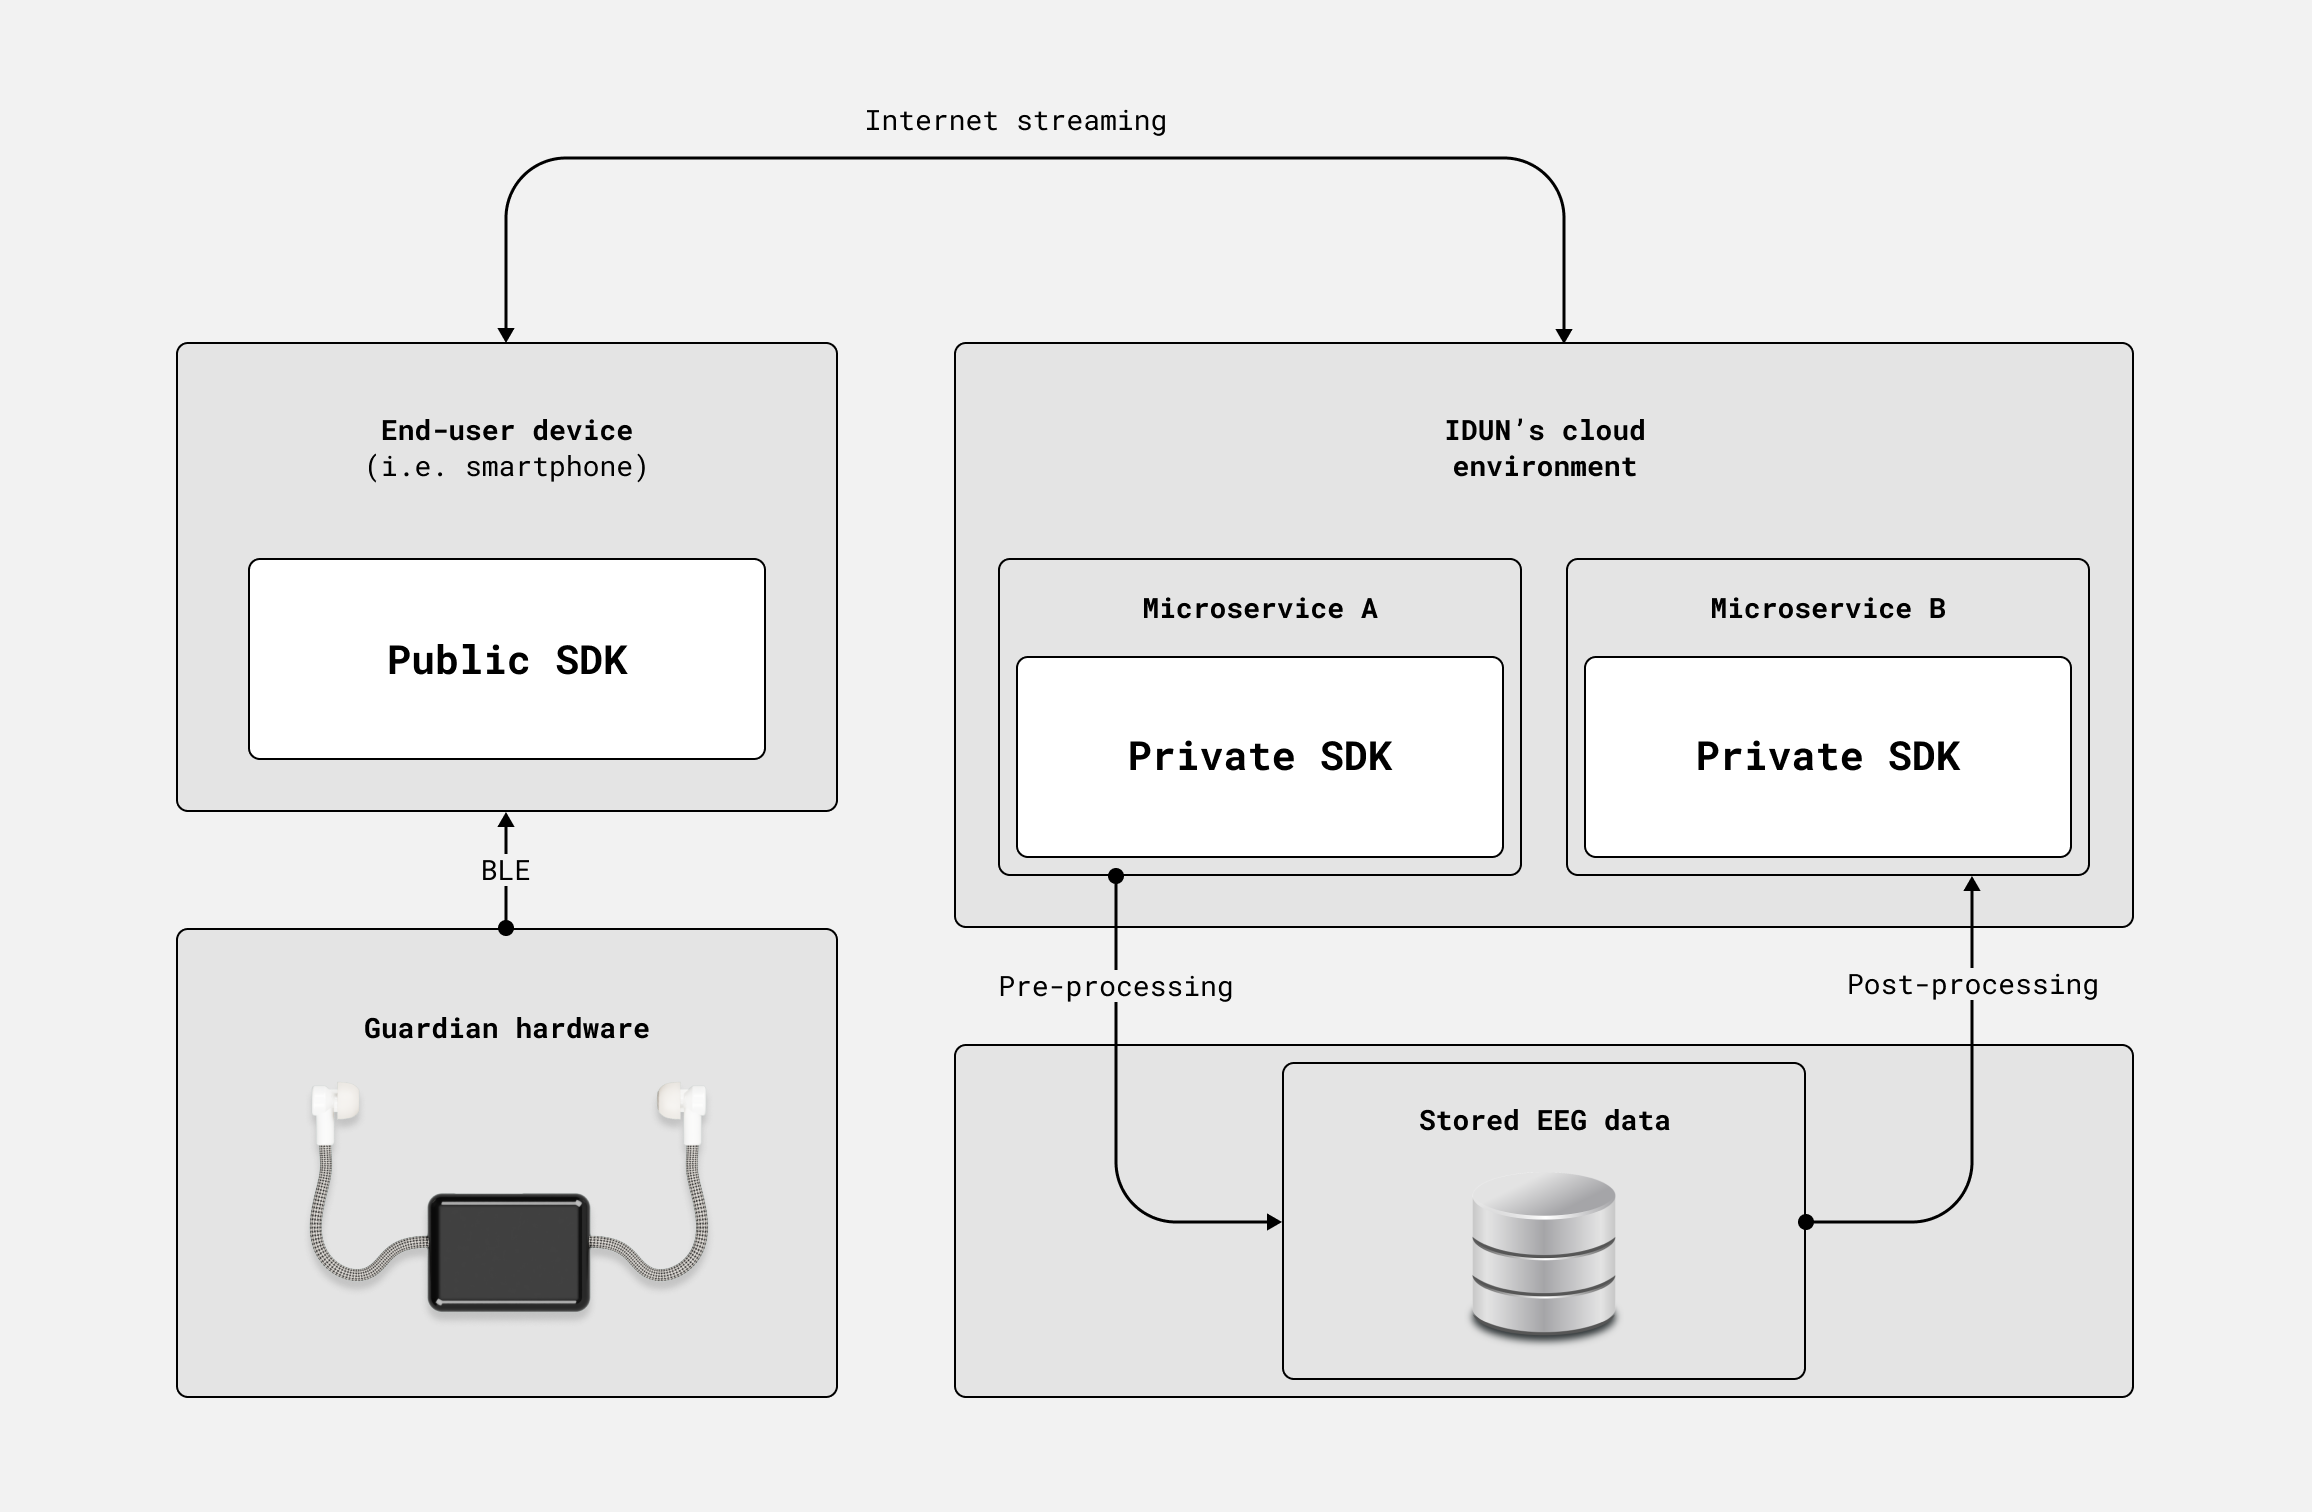
\includegraphics[width=\linewidth]{sdk-overview.png}
  \caption{Overview of where the public and private SDK can be utilised in multiple microservices on the IDUN cloud.}
  \label{fig:sdk-overview}
\end{figure}

Noel would use a GUI application such as the idea for the console application of IDUN’s NIP. However, they would nonetheless still like to have low-level control of the data to include it in PsychoPy experiment scripts or to connect the data via an LSL stream to a reference EEG device to compare EEG signals (which is particularly important for IDUN’s internal researchers).

For this, they would need a library that allows them to connect to the device without an app, if possible, only for research purposes. After the internal group discussions with the neuroscience department, the author proposed building an SDK that does precisely this. Parts of this SDK can also be made public as part of the software offerings from IDUN, such as connecting to a device for limited research purposes or to visualise plots specifically made for IDUN’s EEG data, which was also mentioned as one of the user interview insights in \autoref{chapter4-user-interview-insights}. An internal SDK version of this can be used to include raw data from pre- and post-processing pipelines that are all part of IDUN’s provided intellectual property and should not be made public. Nonetheless, this internal SDK can be used in the neuroscience team and in production—for example, Python microservices that process data on the cloud, as depicted in \autoref{fig:sdk-overview}.

The reason why one would want to have that is that if a data engineer creates new pipeline for processing EEG data that can be used in research or even in production for a microservice, then they would all need to have the exact source of the code. An internal Python package for the SDK is the solution for this. This realisation came fairly late and is, as of this writing, still ongoing.
